\documentclass[twoside, UTF8, a4paper]{ctexart}
\usepackage{array}
\usepackage{graphicx}
\usepackage{geometry}
\usepackage{titlesec}
\usepackage{titletoc}
\usepackage{fancyhdr}
\usepackage{setspace}
\usepackage{amsmath}
\usepackage{amssymb}
%\usepackage{amsfonts}
\usepackage{fontspec}
\usepackage[title, titletoc, header]{appendix}
\usepackage{caption}
\usepackage{enumitem}
\usepackage{booktabs}
\usepackage{listings}
\usepackage{subfigure}
\usepackage{multirow}
\usepackage{hyperref}
% \usepackage{tikz}
% \usepackage[noline]{algorithm2e}

\geometry{top=36mm, bottom=30mm, left=32mm, right=32mm}
\pagestyle{empty}

\ctexset{section={name={第 , 章},format={\center\heiti\zihao{3}\bfseries}}}
\ctexset{subsection={format={\heiti\zihao{4}}}}
\ctexset{subsubsection={format={\kaishu\zihao{-4}}}}

\renewcommand{\abstractname}{\zihao{-3}\bfseries{摘\quad 要}}
\renewcommand{\thefigure}{\thesection{}.\arabic{figure}}
\renewcommand{\thetable}{\thesection{}.\arabic{table}}
\renewcommand{\contentsname}{目\quad 录}
\newcommand{\upcite}[1]{\textsuperscript{\cite{#1}}}
\captionsetup[table]{skip=2pt}
\renewcommand{\thefootnote}{\fnsymbol{footnote}}

\newfontfamily\monaco{Monaco}
\newfontfamily\consolas{Consolas}

\numberwithin{figure}{section}
\numberwithin{table}{section}
\numberwithin{equation}{section}
% \newcommand{\di}{\mathrm{d}}
% \newcommand{\e}{\mathrm{e}}

% \setmainfont{CMU Serif} % for cyrillic and IPA letters

% % algorithm2e package:

% \SetArgSty{textup}

% \makeatletter
% \renewcommand{\@algocf@capt@plain}{above}% formerly {bottom}
% \makeatother

% \renewcommand{\algorithmcfname}{算法}
% \newcommand{\la}{\leftarrow}
% \newcommand{\fnname}[1]{\Indm \ \ #1 \\ \Indp}


% listings package

\lstset{tabsize=4, breaklines=true}

\lstdefinestyle{shared}
{
    backgroundcolor=\color[RGB]{248,248,248},
    basicstyle=\linespread{1.1}\normalsize\consolas,
    frame=l,
    framesep=4pt,
    framerule=0pt
}

\lstdefinestyle{appendix}
{
  basicstyle=\footnotesize\monaco,
  numbers=left,
  numberstyle=\tiny\monaco
}

\hypersetup
{
  colorlinks=true,
  linkcolor=black,
  filecolor=cyan,
  urlcolor=cyan,
  citecolor=cyan,
}

\setlength{\baselineskip}{20pt}
%\setlength{\parskip}{4pt}
\renewcommand\arraystretch{1.2} % linespread in tables
\linespread{1.3}
\setlength{\headheight}{13pt}


\begin{document}

\begin{titlepage}
\newgeometry{top=25mm, bottom=25mm, left=32mm, right=32mm}
\begin{center}
\parskip=0pt

\vspace*{20mm}

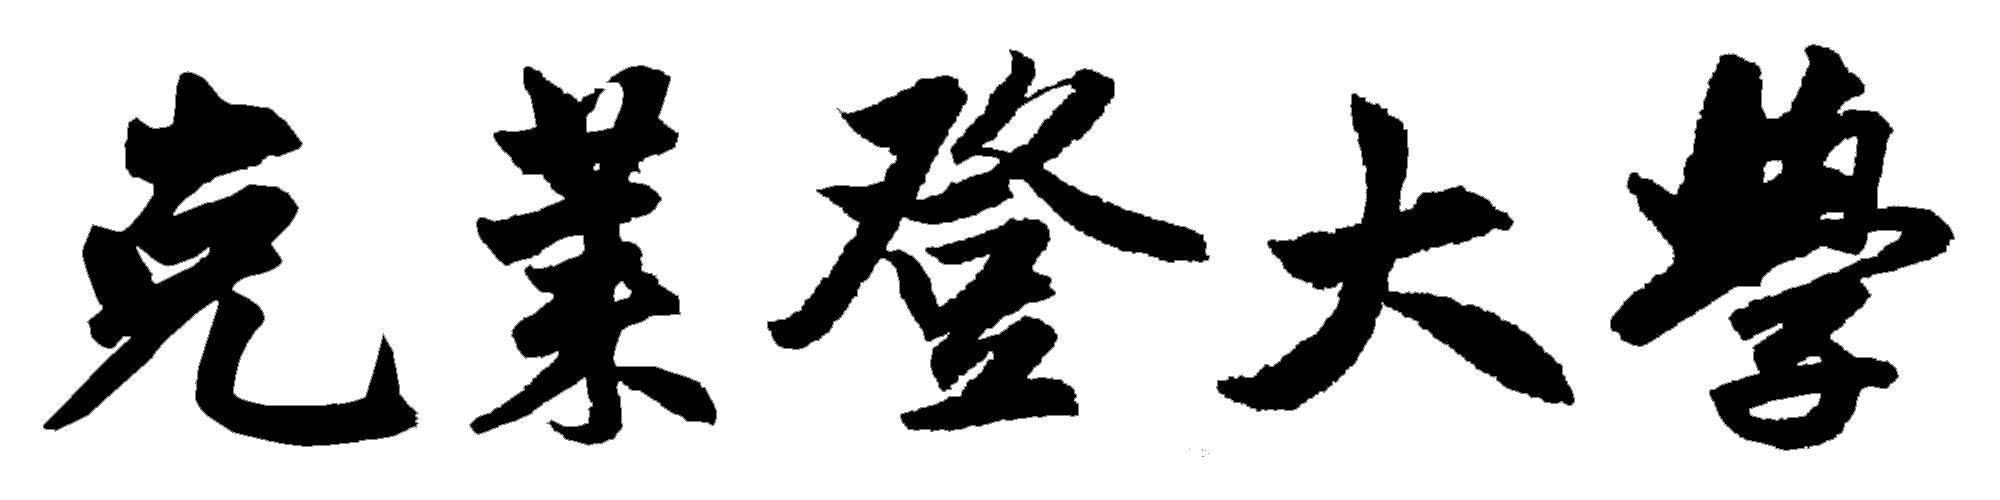
\includegraphics[width=0.6\paperwidth]{./img/claydon-univ-zhaomengfu.png}

\makebox[0.3\paperwidth][s]{\fontsize{14pt}{14pt}\selectfont CLAYDON UNIVERSITY}

\vspace{30mm}

\makebox[0.5\paperwidth][s]{\fontsize{34pt}{34pt}\selectfont\heiti\hspace{0mm}《\,自然辩证法\,》}

\vspace{15mm}

\makebox[0.36\paperwidth][s]{\fontsize{38pt}{38pt}\selectfont\heiti 课程论文}

\vfill

{
\linespread{2}\selectfont
\begin{tabular}{
  >{\centering\fontsize{14pt}{14pt}\selectfont\heiti\arraybackslash}c
  >{\centering\fontsize{14pt}{14pt}\selectfont\fangsong\arraybackslash}p{80mm}
}
  题\qquad 目 & 论非道德意义上的真理与谎言 \\ \cline{2-2}
  学生姓名 & 方鸿渐 \\ \cline{2-2}
  院\qquad 系 & 哲学系 \\ \cline{2-2}
  学\qquad 号 & 2024561414 \\ \cline{2-2}
  指导教师 & Patrick Mahoney \\ \cline{2-2}
\end{tabular}
}

\vspace{25mm}

{
\fontsize{14pt}{14pt}\selectfont
% \the\year 年 \the\month 月
1936 年 7 月
}

\end{center}
\restoregeometry
\end{titlepage}

% \cleardoublepage %---------------------------

\clearpage
\zihao{-4}


\newgeometry{left=4.2cm, right=4.2cm}

\thispagestyle{empty}

\vspace*{15mm}
\begin{abstract}
\zihao{-4}

滚滚长江东逝水,浪花淘尽英雄。是非成败转头空,青山依旧在,几度夕阳红。白发渔樵江渚上,惯看秋月春风。一壶浊酒喜相逢,古今多少事, 都付笑谈中。

\noindent \textbf{关键词:}长江,浪花,英雄,青山,夕阳

\end{abstract}

\restoregeometry

% \cleardoublepage %---------------------------

\clearpage
\zihao{-4}

\clearpage
\setcounter{tocdepth}{3}
\tableofcontents
% \cleardoublepage %---------------------------

\clearpage
\setlength{\parskip}{4pt}
\pagestyle{fancy}
\fancyhf{}
\renewcommand{\headrulewidth}{0.3pt}
%\renewcommand{\footrulewidth}{0.3pt}
\fancyhead[LE]{\leftmark}
\fancyhead[RO]{论非道德意义上的真理与谎言}
\fancyfoot[CF]{\thepage}
\setcounter{page}{1}

\section{Lorem Ipsum}
\subsection{Lorem Ipsum}
\subsubsection{Lorem Ipsum}

Lorem ipsum dolor sit amet, consectetur adipiscing elit, sed do eiusmod tempor incididunt ut labore et dolore magna aliqua. Ut enim ad minim veniam, quis nostrud exercitation ullamco laboris nisi ut aliquip ex ea commodo consequat. Duis aute irure dolor in reprehenderit in voluptate velit esse cillum dolore eu fugiat nulla pariatur. Excepteur sint occaecat cupidatat non proident, sunt in culpa qui officia deserunt mollit anim id est laborum.

\subsubsection{荷塘月色}

这几天心里颇不宁静。今晚在院子里坐着乘凉,忽然想起日日走过的荷塘,在这满月的光里,总该另有一番样子吧。月亮渐渐地升高了,墙外马路上孩子们的欢笑,已经听不见了;妻在屋里拍着闰儿,迷迷糊糊地哼着眠歌。我悄悄地披了大衫,带上门出去。

沿着荷塘,是一条曲折的小煤屑路。这是一条幽僻的路;白天也少人走,夜晚更加寂寞。荷塘四面,长着许多树,蓊蓊郁郁的。路的一旁,是些杨柳,和一些不知道名字的树。没有月光的晚上,这路上阴森森的,有些怕人。今晚却很好,虽然月光也还是淡淡的。

路上只我一个人,背着手踱着。这一片天地好像是我的;我也像超出了平常的自己,到了另一个世界里。我爱热闹,也爱冷静;爱群居,也爱独处。像今晚上,一个人在这苍茫的月下,什么都可以想,什么都可以不想,便觉是个自由的人。白天里一定要做的事,一定要说的话,现在都可不理。这是独处的妙处,我且受用这无边的荷塘月色好了。

\input{essay_content.tex}


\clearpage
\begin{appendices}
\ctexset{section={name={ ,}}}
\section{De Finibus Bonorum et Malorum}

Sed ut perspiciatis, unde omnis iste natus error sit voluptatem accusantium doloremque laudantium, totam rem aperiam eaque ipsa, quae ab illo inventore veritatis et quasi architecto beatae vitae dicta sunt, explicabo. Nemo enim ipsam voluptatem, quia voluptas sit, aspernatur aut odit aut fugit, sed quia consequuntur magni dolores eos, qui ratione voluptatem sequi nesciunt, neque porro quisquam est, qui dolorem ipsum, quia dolor sit amet consectetur adipisci velit, sed quia non numquam eius modi tempora incidunt, ut labore et dolore magnam aliquam quaerat voluptatem. Ut enim ad minima veniam, quis nostrum exercitationem ullam corporis suscipit laboriosam, nisi ut aliquid ex ea commodi consequatur? Quis autem vel eum iure reprehenderit, qui in ea voluptate velit esse, quam nihil molestiae consequatur, vel illum, qui dolorem eum fugiat, quo voluptas nulla pariatur?

\begin{figure}[!ht]
\centering
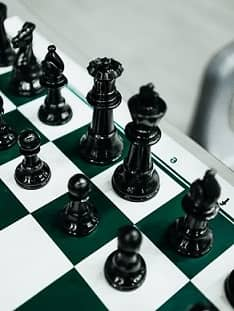
\includegraphics[width=0.3\linewidth]{./img/black-chess-pieces.jpg}
\caption{This image is in the public domain}
\label{fig:black-chess-pieces}
\end{figure}

\clearpage
\section{Spacewar!}

\begin{lstlisting}[style=appendix]
MOVEI P,PDL
CONO 633550+APRCHN
CONO PI,12207
SETZM BKTMF'
SETZM BKTIME'
SETZM BKTS'
SETZM BKX'
MOVE A,BKSTP
MOVEM A,BKSTRT'
SETZM RE1'
SETOM SCNDF'
CLEARM SCOREF'
MOVEI A,SDISE-1
MOVEM A,DISPNR
MOVE A,SSBRI
MOVEM A,SDIS
CONO DIS,100+FLGCHN_3+DISCHN
\end{lstlisting}

\end{appendices}


\clearpage
\begin{flushleft}
\begin{thebibliography}{0}
\addcontentsline{toc}{section}{参考文献}
\kaishu\zihao{5}
\bibitem{} Xueyu Han. (1929) On Truth and Lies in a Nonmoral Sense. PhD thesis. Claydon University.
\end{thebibliography}
\end{flushleft}

\end{document}
